% Este archivo es parte de la memoria del proyecto fin de carrera
% de Manuel López Urbina. Protegida bajo la licencia GFDL.
% Para más información, la licencia completa viene incluida en el
% fichero fdl-1.3.tex

% Copyright (C) 2018 Manuel López Urbina

\newpage

\chapter{ Pruebas }
\label{chap:pruebas}

La realización de pruebas de software, es una de las fases del ciclo del software de gran importancia, la cual permite la identificación de posibles fallos en la implementación, 
calidad o usabilidad de la aplicación con la finalidad de que el producto final cumpla una serie de garantías y sea de calidad.\\

\section{Plan de pruebas}

Debido a la arquitectura de SensorRS y a la metodología basada en desarrollo incremental que se ha seguido en el desarrollo y construcción del proyecto robótico,
se ha establecido un plan de pruebas en el que las diferentes partes han ido siendo analizadas y testeadas de forma independiente. La aplicación y el robot ha sido sometido 
a una batería de pruebas. 

Una vez finalizado el proceso de montaje y control, las pruebas que se realizaron para comprobar el vehículo cumplía con los requisitos propuestos en su diseño fueron las siguientes:\\

\begin{description} 

\item [Pruebas de funcionamiento:]\\

\begin{itemize}
    \item[]
 \item Se controla que los diferentes elementos y componentes electrónicos se encuentran correctamente alimentados y con un conexionado lo suficientemente fuerte y estable 
 para que no de lugar a posibles fallos tras someter al vehículo a los movimientos ocasionados por su uso.
\end{itemize}


\item [Pruebas de comunicaciones:]\\

\begin{itemize}
    \item[]
 \item Se comprueba que se realiza una comunicación correcta entre la placa Arduino - Raspberry Pi y entre Raspberry PI - Servidor sometiendo al sistema a situaciones de tráfico elevado
 y analizando su comportamiento.
\end{itemize}


\item [Pruebas de control:] \\

\begin{itemize}
    \item[]
 \item Se comprueba que se realiza un manejo adecuado del dispositivo robótico.
 \item Se comprueba que se obtiene y muestra correctamente las diferentes mediciones obtenidas de los sensores comparando los resultados medidos con sensores externos al vehículo o comparando
 las las distancias obtenidas con la realización de mediciones con una cinta métrica. 
\end{itemize}


\item [ Pruebas de alcance:] \\ 

\begin{itemize}
    \item[]
 \item Se somete al vehículo a una prueba de alcance bordeando de la zona de cobertura abarcada por el punto de acceso wifi en el que el vehículo se encuentra conectado obteniendo un
 resultado satisfactorio en distancias superiores a los 15 metros.
\end{itemize}

\item [ Pruebas de pista:] \\ 

\begin{itemize}
    \item[]
 \item Se somete al vehículo a una prueba de movimientos por diversos tipos de pista, asfalto, hormigón tierra comprobando que se desenvuelve con soltura a todas las situaciones mencionadas.
\end{itemize}


\begin{figure}[H]
    \centering
    \begin{subfigure}[b]{0.4\textwidth}
        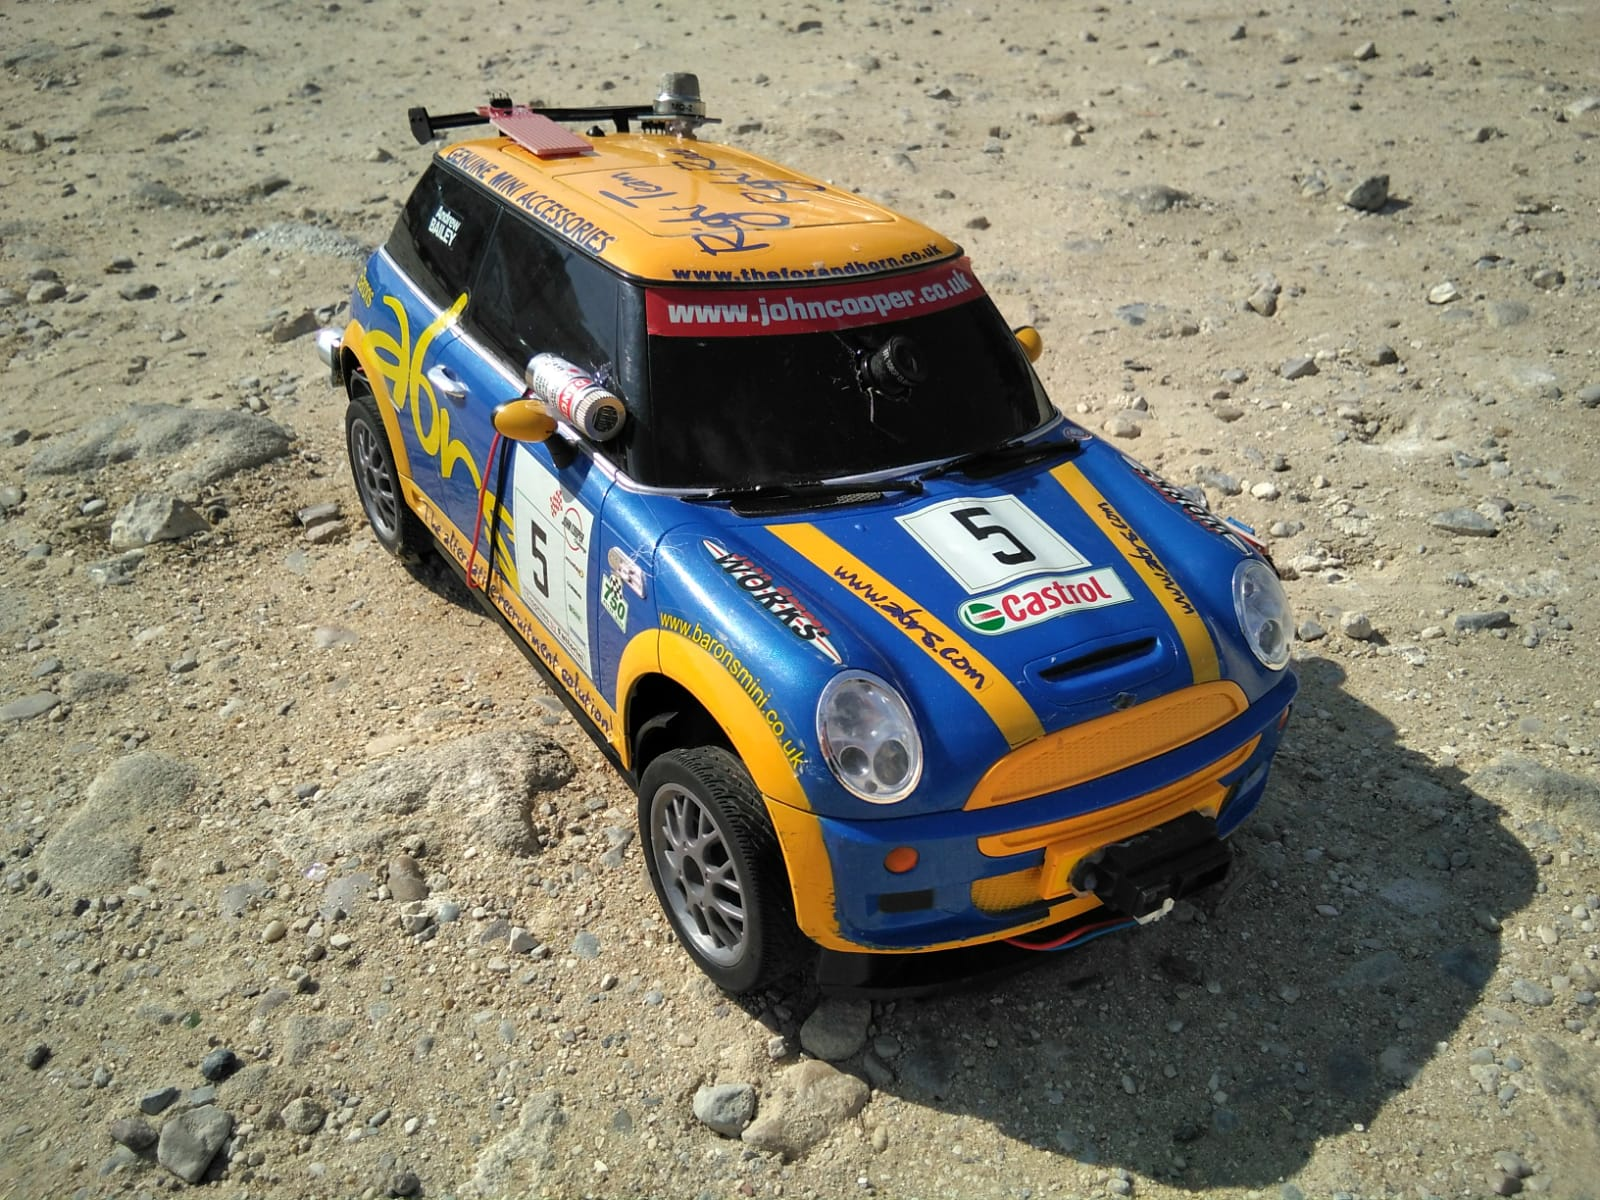
\includegraphics[width=\textwidth]{imagenes/robot/tierra.jpg}
        \caption{Pista de tierra.}
        \label{fig:gull}
    \end{subfigure}
    \begin{subfigure}[b]{0.4\textwidth}
        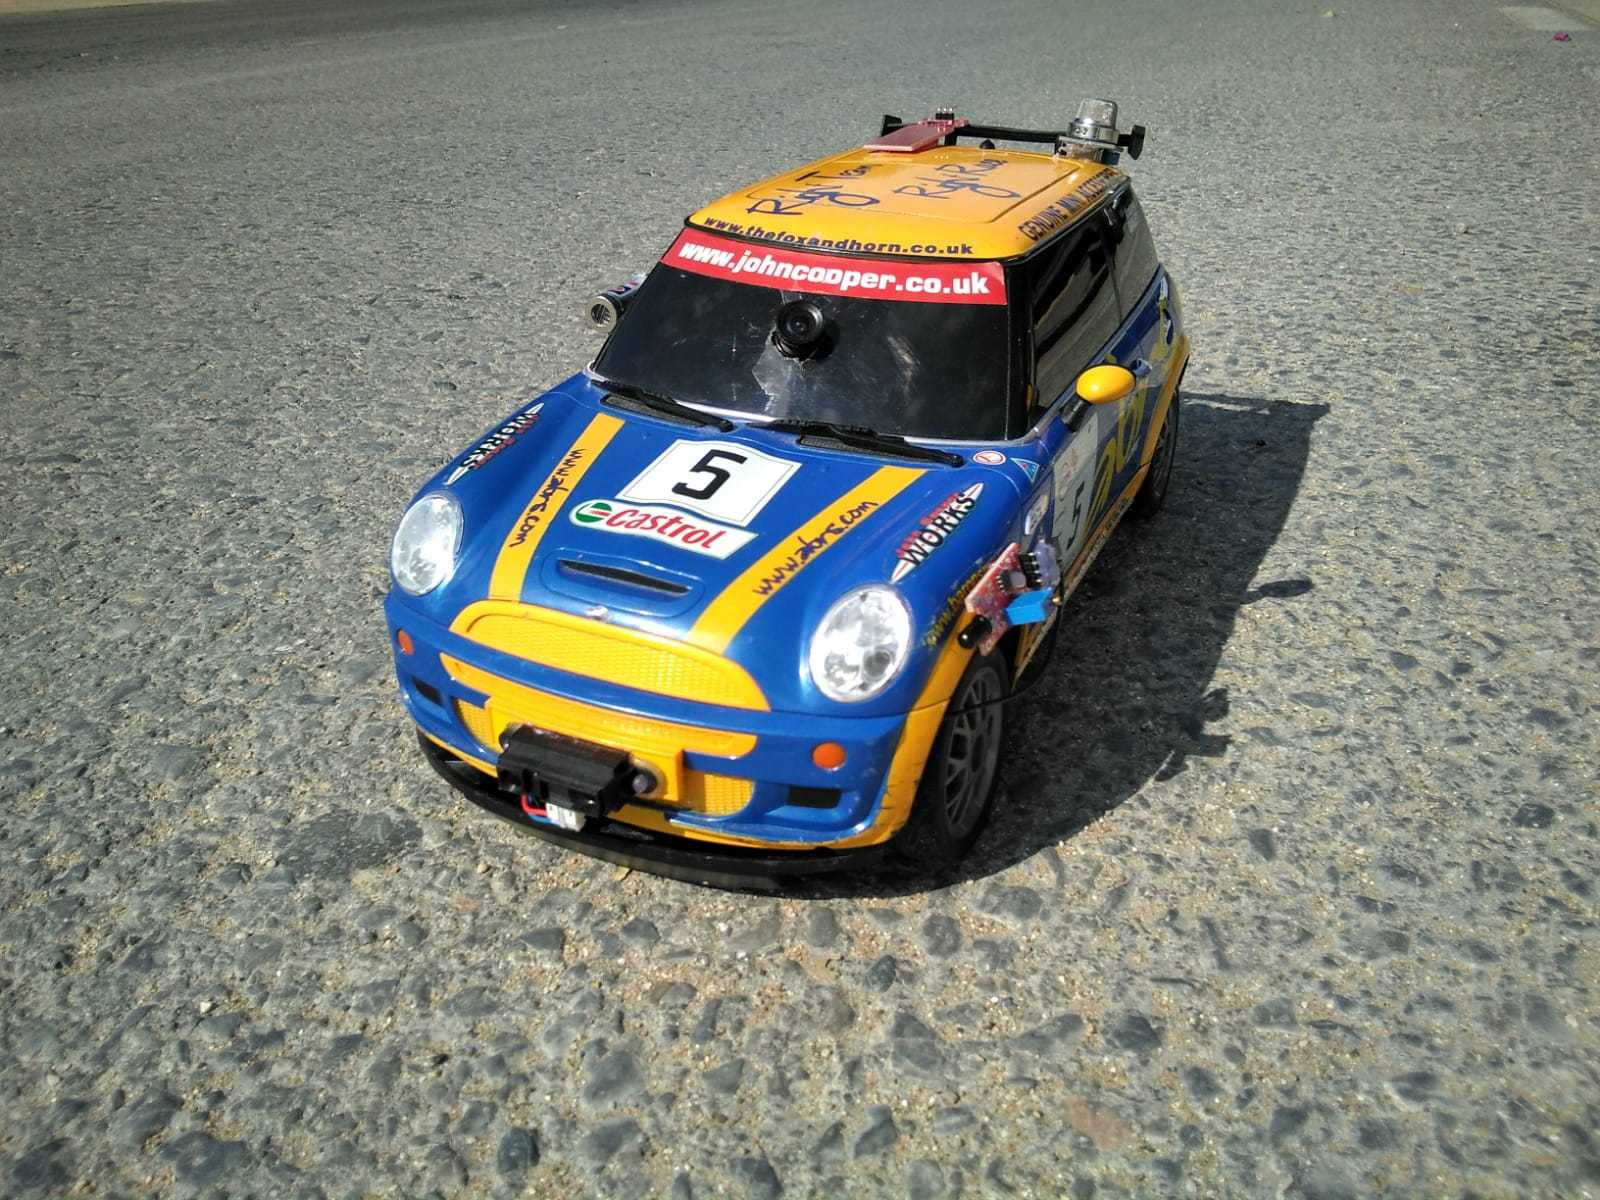
\includegraphics[width=\textwidth]{imagenes/robot/asfalto.jpg}
        \caption{Pista de asfalto.}
        \label{fig:tiger}
    \end{subfigure}
    \begin{subfigure}[b]{0.4\textwidth}
        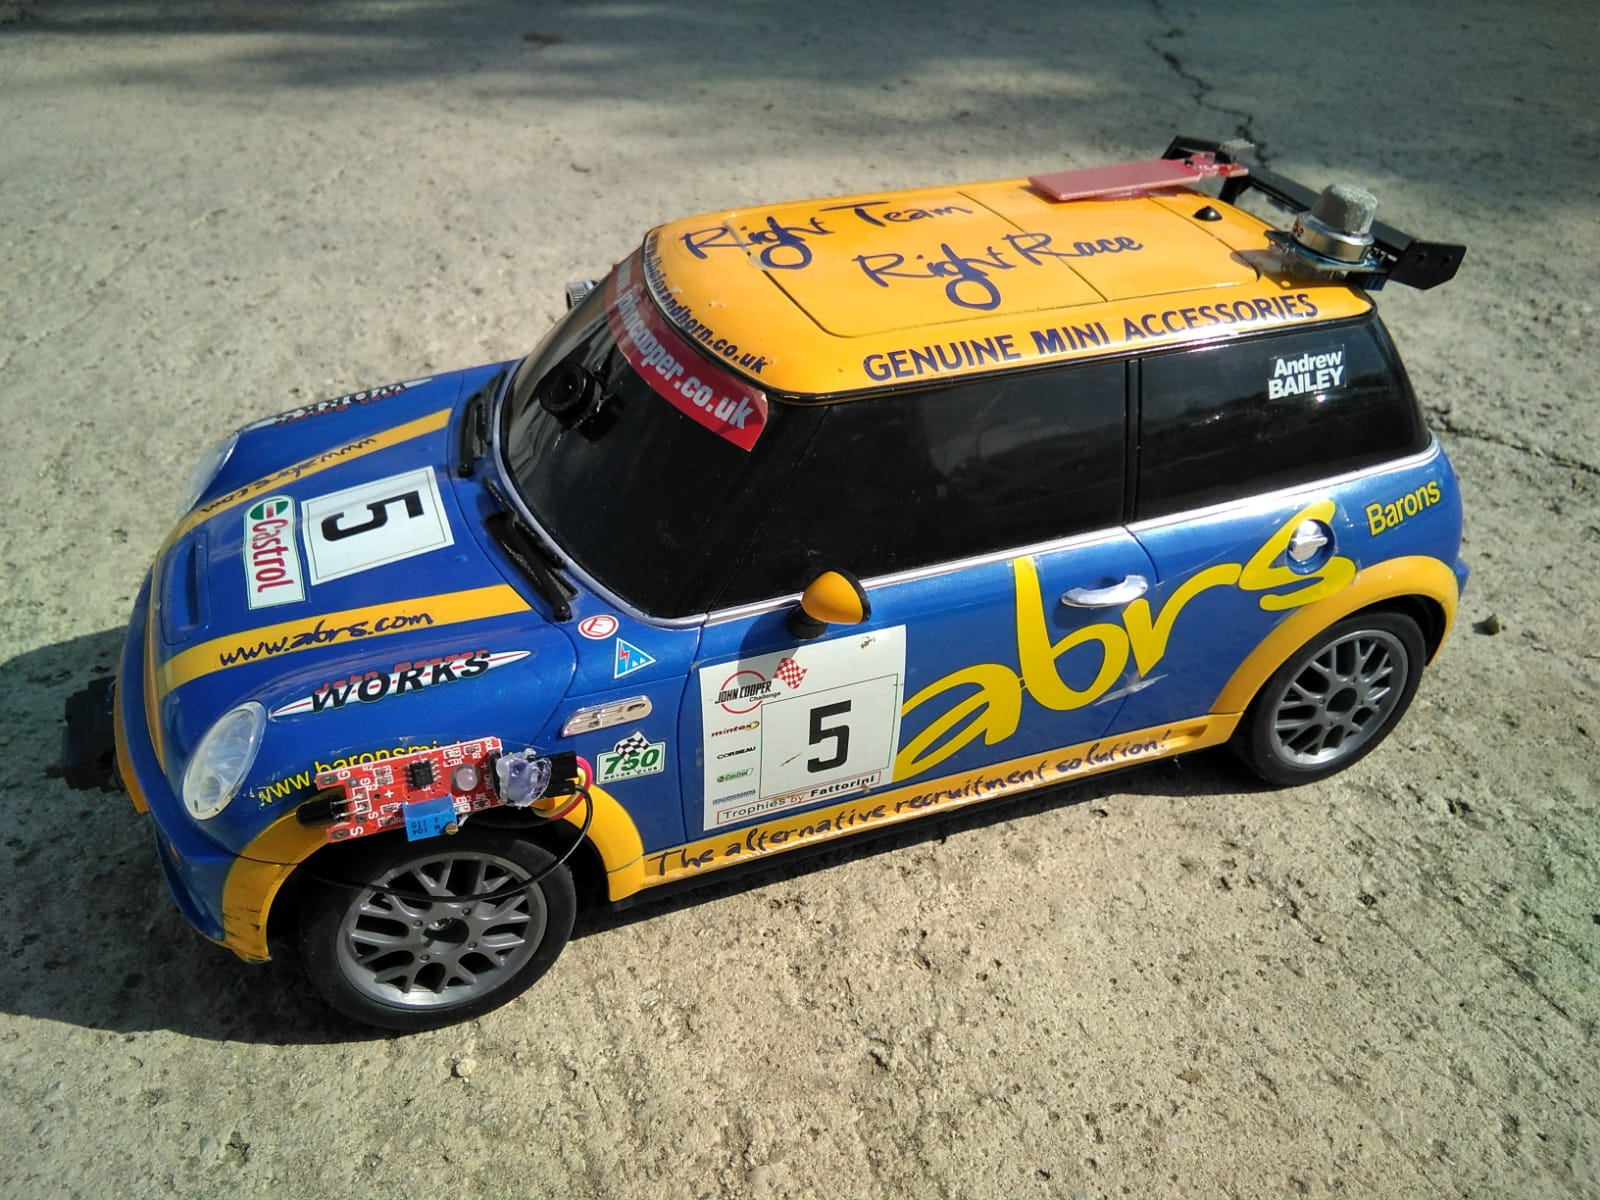
\includegraphics[width=\textwidth]{imagenes/robot/hormigon.jpg}
        \caption{Pista de hormigón.}
        \label{fig:mouse}
    \end{subfigure}
    \caption{Vehículo SensorRS en funcionamiento por diferentes tipos de pista.}\label{fig:animals}
\end{figure}

\end{description}



